\documentclass{article}

% Language setting
% Replace `english' with e.g. `spanish' to change the document language
\usepackage[english]{babel}

% Set page size and margins
% Replace `letterpaper' with `a4paper' for UK/EU standard size
\usepackage[letterpaper,top=2cm,bottom=2cm,left=4cm,right=4cm,marginparwidth=2.5cm]{geometry}

% Useful packages
\usepackage{amsmath}
\usepackage{graphicx}
\usepackage[colorlinks=true, allcolors=blue]{hyperref}

\title{CS307 Database project part1}
\author{Name: Wen Yinan\\
StudentID: 12310841\\
\vspace{1em} % 插入空行
Class#: Lab Mon 9-10\\
Name: Cui Zixuan\\
StudentID: 12311007\\
Class#: Lab Mon 9-10
}

\begin{document}
\doublespacing
\maketitle
\newpage
\tableofcontents

\section{Information and Contribution}
\subsection{Contribution}

The basic information and contribution of our members are as follow.

\subsection{Language}

We applied the following languages in our design\\
    Java 19.0.1 2022-10-18\\
    Java(TM) SE Runtime Environment (build 19.0.1+10-21)\\
    Java HotSpot(TM) 64-Bit Server VM (build 19.0.1+10-21, mixed mode, sharing)\\

 \subsection{Test Environment}
We deployed two machines in our test\\
• HUAWEI SOUND(Processor: 13th Gen Intel(R)Core(TM)i5-13500H 2.60 GHz)\\
 • Lenovo Legion R9000x-2021-R(Processor: AMD Ryzen 7 5800H with Radeon Graphics            3.20 GHz)
\section{ER Diagram}
\subsection{Designing the E-R Diagram}
 This section outlines the methodology and tools used to design the ER diagram
 for our video website. Additionally, it provides a visual representation of the
 ER diagram.
 \subsubsection{Methodology}
  To design the ER diagram, we followed a systematic methodology:\\
 1. Identify Entities and Attributes:- We identified the main entities in our database, such as Users, Videos, and
 Danmu. For each entity, we determined the relevant attributes, like User ID,
 Video Title, and Danmu Content.\\
 2. Define Relationships:- we focus on the relationships between entities and attributes, and see how they
 connect.\\
 3. Constraints:- Weassigned constraints to relationships to specify the nature of the connection
 between entities.\\
 4. Normalization:- We ensured that the ER diagram followed the principles of normalization to
 minimize redundancy and improve data integrity.
\subsubsection{Tools Used}
We used draw.io to create our ER diagram. Draw.io allows us to easily represent the entities, attributes, and relationshipswithin our database model.
\newpage
\subsubsection{ER Diagram Snapshot}
Below is a snapshot of the ER diagram we designed for our website:

\begin{figure}[h]
\centering % 确保图片居中显示
\includegraphics[width=.8\textwidth]{ER图.png} % 插入图片并调整大小
\caption{ER Diagram} % 为图片添加描述性标题
\label{fig:引用标签} % 为图片分配一个引用标签,方便后续引用
\end{figure}
 

This ER diagram visually represents the entities, their attributes, and the relationship between them
\subsection{Entities and Attributes}
In this ER diagram, we can visually identify all the entities, attributes, and relationships. The entities include "article","author","journal","grant","publication types","article ids" and ”references” The attributes for each entity are as follows:
\subsubsection{Article}
\setlist 
\begin{mylist}  
 \item \textbf{Entity:} Article
 \item \textbf{Attribute:}
  \item - id  
  \item - title  
  \item - data created
  \item - data completed
  \item - keywords
  \item - pub model
\end{mylist} 

\subsubsection{Author}
\setlist 
\begin{mylist}  
 \item \textbf{Entity:} Author
 \item \textbf{Attribute:}
  % \item - author id
  \item - lastname  
  \item - forename  
  \item - collective name 
  \item - affaliations 
  \item - initials  
\end{mylist}  


\subsubsection{Journal}
\setlist 
\begin{mylist}  
 \item \textbf{Entity:} Journal
 \item \textbf{Attribute:}
  \item - journal id  
  \item - title  
  \item - country
  \item - issn
  \item - journal issue volume
  \item - journal issue issue
  
\end{mylist}  

\subsubsection{Grant}
\setlist 
\begin{mylist}  
 \item \textbf{Entity:} Grant
 \item \textbf{Attribute:}
  \item - grant id  
  \item - agency  
  \item - country
  \item - acronym
\end{mylist}  

\subsubsection{References}
\setlist 
\begin{mylist}  
 \item \textbf{Entity:} References
 \item \textbf{Attribute:}
  % \item - article id  
  \item - reference id  
\end{mylist}  

\subsubsection{Publication Types}
\setlist 
\begin{mylist}  
 \item \textbf{Entity:} Publication Types
 \item \textbf{Attribute:}
  \item - article id  
  \item - publication types id  
\end{mylist}

\subsubsection{Article id}
\setlist 
\begin{mylist}  
 \item \textbf{Entity:} Article id
 \item \textbf{Attribute:}
  \item - id
  \item - article id  
  \item - reference id  
\end{mylist}  

\subsubsection{Relationships}
In this diagram, we can clearly observe the relationships between different attributes. For example, the relationship between ”article” and ”author”
is denoted as ”written by,” indicating that the article is written by a author with a specific author id. Another example is the relationship between ”article” and
”journal”, signifying that article is published in a journal with a unique journal id.
This ER diagram provides a comprehensive view of the structure of the
database and how entities and attributes are interconnected.



\section{Database Design}
\subsection{Raw Data}
The data file is pubmed24n.ndjson
\subsection{Design}
\subsubsection{Analysis}
In this part, we delved into the provided data files and their structures, aiming
to identify the primary entities, attributes, and define the relationships between
them.

\textbf{Entity Identification:}  we identified the main entities that would form the
basis of our database. These entities include ”users,” ”videos,” and ”danmu.”

\textbf{Attribute Identification:}  For each entity, we recognized the associated
attributes. For example, in the ”users” entity, attributes such as ”mid,” ”name,”
”sex,” and others were identified.

\textbf{Relationship Definition:}  We explored the relationships between entities.
For example, we related the entity "grant","publication type", and "journal id" to the corresponding article id.

\textbf{Data Normalization:}  We ensured that our database design adhered to the principles of normalization. In the subsequent sections, we will delve into
this aspect in greater detail.
\\ [1.3ex]
Through this analysis phase, we laid the foundation for the database design by identifying data entities, attributes, and relationships, ensuring that the
structure of the database aligns with the project requirements. The subsequent sections will delve deeper into the specific structure and constraints of the database
\subsubsection{Structure}
Within this section, we created seven main tables and three auxiliary tables.
The main tables are "article","author","journal","grant","references","publication type" and "article id"  while the auxiliary tables
include "article-author","article-publication-type" and "article-grant" tables. Let me introduce each of the main and auxiliary tables individually.

\begin{itemize}
\item \textbf{Article Main Table}
\begin{enumerate}
\item \textbf{id(int, PRIMARY KEY, unique)}
\item \textbf{title(varchar(2550),not null):} We used the varchar(2550) data type for "title" to ensure it can accommodate sufficiently long article titles
\item \textbf{pub model(varchar(30)):} We utilized the varchar data type for ”pub model” as there are only five possible values for it : "Print" , "Print-Electronic" , "Electronic" , "Electronic Print" , "Electronic-eCollection".
\item \textbf{date created(date, not null):} We use the date data type for the DATE type ensures that date data is stored in a uniform format (YYYY-MM-DD), avoiding errors caused by inconsistent formats. Also by using the DATE type, the stored dates can be limited to a reasonable range, preventing the input of invalid dates such as "2024-13-01". Moreover, Using the DATE type can reduce unnecessary storage space usage, especially when dealing with large amounts of date data.
\item \textbf{date completed(date):} It is very similiar to the colume "date created".
\item \textbf{keyword(varchar(2550)):} The varchar(2550) data type is used for ”keyword” to ensure it can accommodate sufficiently long keyword.
\item \textbf{journal varchar(50):} The journal id here is linked to the journal id in the journal table
\end{enumerate}

\item \textbf{Author Main Table}
\begin{enumerate}
\item \textbf{author id(serial PRIMARY KEY):} We choose serial as its datatype to create a unique primary key. It ensures each relationship
has a unique identifier, and the identifier increments automatically, making it easy to manage.
\item \textbf{lastname(varchar(70))}
\item \textbf{forename(varchar(30))}
\item \textbf{initials(varchar(30))}
\item\textbf{affiliation(varchar(1000))}
\item \textbf{collective name(varchar(1000))}  
\end{enumerate}


\item \textbf{Journal Main Table}
\begin{enumerate}
\item \textbf{journal id(varchar(40) PRIMARY KEY}
\item \textbf{title(varchar(2550),not null)}
\item \textbf{country(varchar(100))}
\item \textbf{issn(varchar(20))}
\item \textbf{journal-issue-issue(varchar(200))}
\item \textbf{journal-issue-volume(varchar(200))}
\end{enumerate}


\item \textbf{Grant Main Table}
\begin{enumerate}
\item \textbf{grant id(varchar(50) PRIMARY KEY):}
\item \textbf{agency(varchar(255) not null):} We used the varchar(255) data type for ”agency” to ensure it can accommodate sufficiently long agency name.
\item \textbf{country(varchar(70))}
\item \textbf{acronym(varchar(50))}
\end{enumerate}


\item \textbf{Reference Main Table}
\begin{enumerate}
\item \textbf{article id(int PRIMARY KEY):} It is linked to the article id in article table.
\item \textbf{reference id(varchar(50),PRIMARY KEY)}
\end{enumerate}

\item \textbf{Article Ids Main Table}
\begin{enumerate}
\item \textbf{article id(int PRIMARY KEY)}
\item \textbf{id(varchar(100))}
\item \textbf{type(varchar(10) PRIMARY KEY)}
\end{enumerate}

\item \textbf{Publication Type Main Table}
\begin{enumerate}
\item \textbf{publication type id(varchar(50) PRIMARY KEY):}
\item \textbf{name(varchar(50))}
\end{enumerate}
\end{itemize}

\begin{itemize}
\item \textbf{article-author Table,article-publication-type Table,article-grant Table:} This four tables share similar structures, aiming to connect the article with author, article with publication type, and article with grant by their id.
\begin{enumerate}
\item \textbf{article id(int PRIMARY KEY)}
\item \textbf{author/publication type/grant id(int PRIMARY KEY)}
\end{enumerate}


\end{itemize}
\subsubsection{Scalability }

\textbf{Scalability Overview}
Scalability in system design refers to the ability to easily add new features and handle changes without impacting performance. In this project, the focus is on enabling easy feature extensions, as the data volume isn’t large.\\

\textbf{Scalability Through Diagram Design}
\begin{itemize}
\item Modular Class Design
The system is designed with separate classes for different tasks (e.g., DatabaseManager, DataInsert, AuthorInsert). This modular approach allows adding new features (like new data types) without disrupting existing functionality.
\item Database Abstraction
Database interactions are abstracted, ensuring that database changes (e.g., switching from relational to NoSQL) don’t affect the rest of the system. The separation of data models from database logic enables easy modifications or additions.
\item Flexibility to Add Features
New use cases or features can be integrated easily into the system without major changes, thanks to clear data flow paths and extensible classes.
\item Clear Data Relationships
The ER diagram defines clear relationships between entities (e.g., Author, Article), making it easy to add new entities or relationships when needed.
\item Extensibility with Data Sources
The sequence diagram allows for the easy addition of new data sources (e.g., XML or API) without disrupting existing processes.

\end{itemize}
\textbf{Conclusion:}
The system’s design ensures scalability by using modular components, abstracted database interactions, and flexible data relationships, making it easy to add new features and data sources in the future.

\subsubsection{Normalization}

\textbf{\uppercase\expandafter{\romannumeral+1} Normalization in Our Design}
\begin{itemize}
    \item\textbf{ 1NF (First Normal Form)} Fields must be atomic and cannot contain sets or lists. 
    
    In our design, all tables are atomic, and each table’s attributes are atomic. For example, We separated the author, grant, journal, and reference related to article into new tables. As a result, there are no shared components between any two tables, except for the primary key article-id they both depend on.
    \item\textbf{ 2NF (Second Normal Form)} Eliminate partial dependency, ensuring non-primary key fields fully depend on the primary key.
    
    In our design, all non-primary key fields fully depend on the primary key. They do not depend on any other table's primary key. A non-primary key would not depend on the primary key if it is not related to it directly. In our table design, We categorized all attributes parsed from the NDJSON file and designed tables for each one, effectively avoiding this issue.
    \item\textbf{ 3NF (Third Normal Form)}Eliminate transitive dependency, ensuring non-primary key fields do not depend on other non-primary key fields. 
    
    In our tables, non-primary key fields depend only on the primary key. For example, in the article table, fields like id, title, date-created, date-completed, pub-model, and keyword do not depend on other non-primary key fields. They only depend on the primary key id.
 that non-key attributes do not depend on other non-key attributes within
 the same table
\end{itemize}
\textbf{\uppercase\expandafter{\romannumeral+2} Minimizing Data Redundancy}

This database design minimizes data redundancy by carefully separating the data into distinct tables. For example, each table stores only the relevant attributes, and no data duplication occurs between tables. This helps in reducing redundancy, improving data integrity, and simplifying data maintenance.

Each table is represented by a specific class in our codebase, with distinct methods to handle parsing and inserting data into the tables. For instance, the Article, Jouranl, Grant, Followings, author, reference, publicaitonType, and articleGrant tables each have a corresponding class and method that parses data and inserts it into the database.

A central DataManager class handles database connections, ensuring all database operations are done through a single connection. This reduces the complexity of managing multiple database connections.

The DataInsert class is responsible for the logic of inserting parsed data into the appropriate tables, using batch inserts for efficiency and ensuring that the data is correctly formatted and validated before insertion.
\vspace{6pt}
\\
\textbf{\uppercase\expandafter{\romannumeral+3} Conclusion of Normalization}

In conclusion, this database design follows the principles of normalization, reducing data redundancy and improving data integrity. The separation of data into distinct tables, as well as the use of primary keys to uniquely identify records, ensures the database adheres to the three normal forms (1NF, 2NF, and 3NF). This structure not only enhances data integrity but also ensures that our system can be easily expanded with additional features while maintaining performance.
% \newpage
\newpage
\subsection{Conclusion}
Here is the database diagram for a clearer understanding of our database design.

\begin{figure}[h]
\centering % 确保图片居中显示
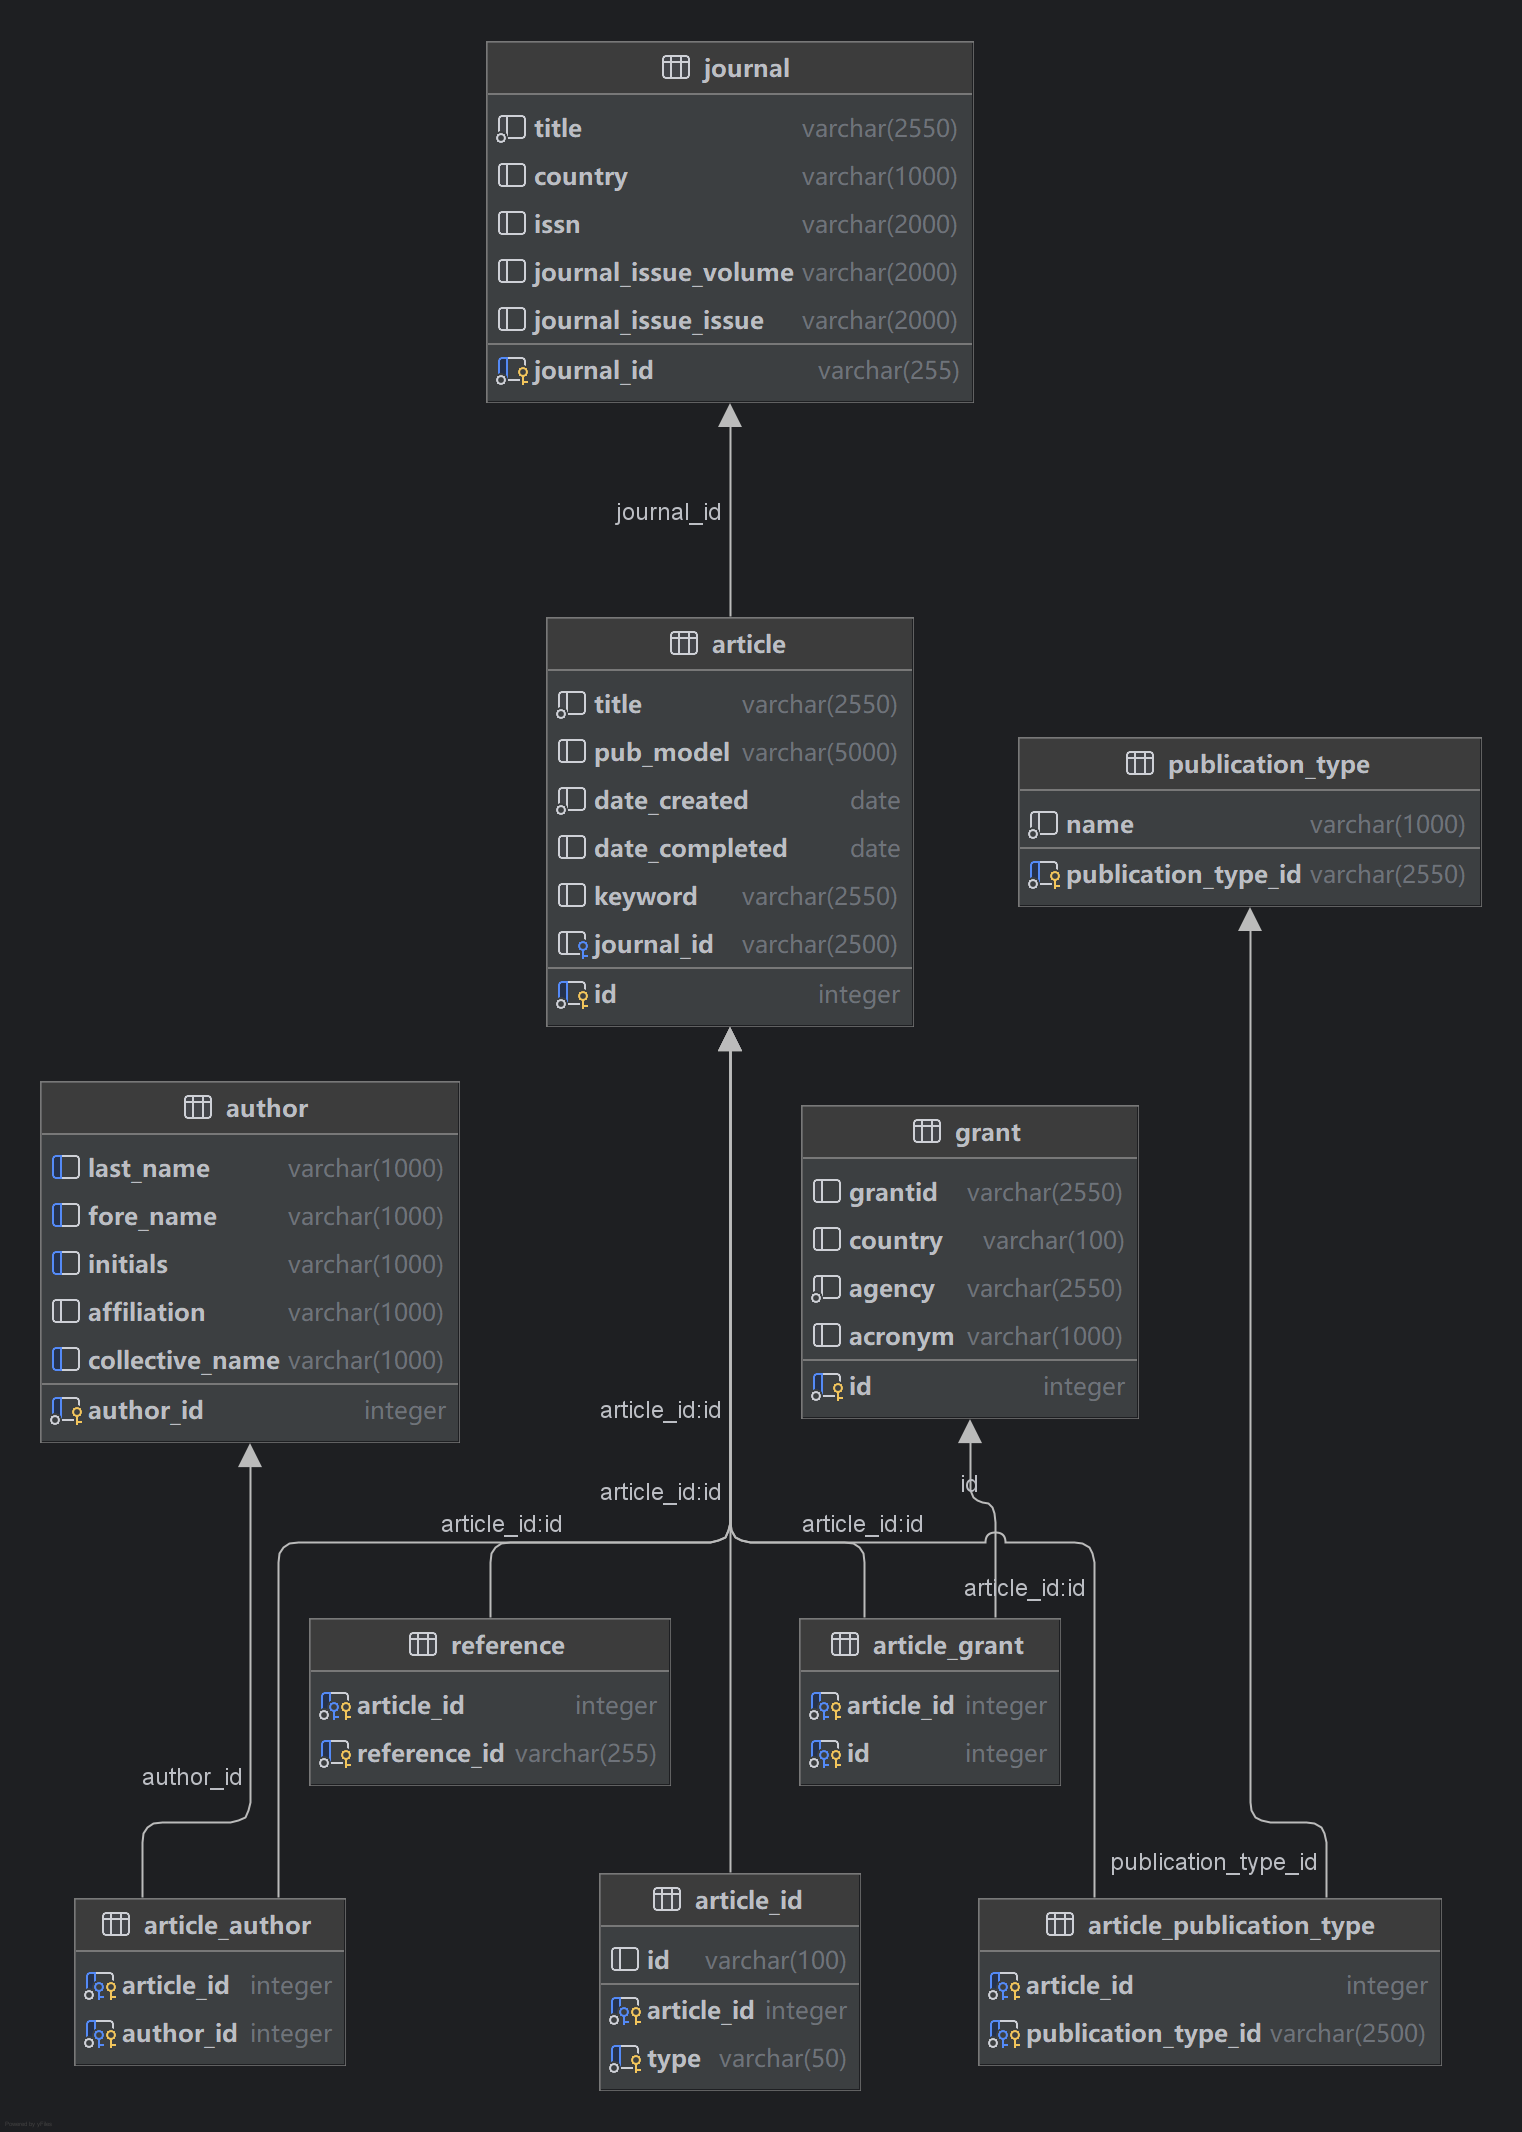
\includegraphics[width=.8\textwidth]{logic.png} % 插入图片并调整大小
\caption{ER Diagram} % 为图片添加描述性标题
\label{fig:引用标签} % 为图片分配一个引用标签,方便后续引用
\end{figure}




\section{Data Import}
In this part, we’ll offer a guidance to run our import scripts. Next, an explanation of the principles of the scripts will be given. However, since the average method has a relatively low efficiency, we’ll introduce a way to enhance the
process. The strategies include
\begin{itemize}
    \item\textbf{ Optimize the database design}
    \item\textbf{ Deleting Unnecessary checks}
    \item\textbf{ Batch Processing}
    \item\textbf{ Use the transaction of PostgreSQL}
\end{itemize}
We also used Python to write a script for importing the data, and we made a comparison of this method with the traditional Java Database Connectivity method.
\subsection{Guidance}
\subsubsection{Prerequisite}
To run our scripts, you should have these installed at first
\begin{itemize}
    \item\textbf{ Java 17}
    \item\textbf{ IntelliJ IDEA 2024.2.1 and Intellij IDEA 2024.2.4}
    \item\textbf{ Postgres 15}
    \item\textbf{ JDBC PostgreSQL (Maven)}
    \item\textbf{ Python 3.7}
    \item\textbf{ Python charm 2019.2.4}
    \item\textbf{ Datagrip2024.2.2}
\end{itemize}
 % We also provide a user-friendly option that uses IntelliJ IDEA to run the program, which can be accessed through \href{https://github.com/chanbengz/SUSTech_CS307_2023F_Project1}{https://github.com/chanbengz/SUSTech_CS307_2023F_Project1}
\subsubsection{Create Database}
Then follow these steps to configure your database
\begin{enumerate}
\item Open your Datagrip and click the File option and you will find a new option, make your mouse hanging on the New option and you will will find a DataSource option in the new line showned.
\item Click the DataSource option and choose the PostgresSQL option and click.
\item In the new window named DataSource and divers, edit the username and your password to finish the last step.
\item Click the Test Connection button to ensure you have down load the necessary diver.
\item Open our IDEA java codes and enter the Main class, change the file path into yours. And enter the Datamanager class just change the URL, Username, and the password.
\item Till now, you can cilick the Main button and run the codes to import Data!!!
\end{enumerate}
\subsubsection{Notice}
 Remember to change the username and password in the connect method of
 the script. And make sure there is a ndjson file in your path which has been changed by yourself.
\subsection{Design}
\subsubsection{Code}
 The source code is the DBMS.zip in the submitted zip file.
%  can be reached by \href{https://github.com/chanbengz/SUSTech_CS307_2023F_Project1}{https://github.com/chanbengz/SUSTech_CS307_2023F_Project1} in the archive.
\subsubsection{Principles}

\begin{enumerate}
\item Connect to the Database\\
The script starts by establishing a connection to the PostgreSQL database. The DatabaseManager class is responsible for managing the database connection, handling connection opening, maintaining the connection, and closing it.
\item Import Data
\begin{itemize}
\item Parese the ndjson file
\item Create class
\item Import different data into the corresponding tales
\item Commit
\end{itemize}
\item Close the Database Connection
\end{enumerate}


 In the script, the steps are executed one after one by the order in single thread.\\
 In each import method, we firstly parse one line of the ndjson file, and in the DataInsert class, we parse the data from the ndjson file into different parse methods, and then we have a corresponding insert method for each parse method. Then the data has been imported.

\subsection{Result and Analysis}
The result of successful import is
\begin{table}[h!]
\centering
 \begin{tabular}{c c c c c c c c} 
 \hline
\textbf{Tablename} & Article & Author & Journal & Grant & Publication type & Reference & Article-ids\\ [0.1ex] 
 \hline 
 \\[0.00000000001ex]
 \textbf{Records} & 3000000 & 1671875 & 5639 & 388146 & 50 & 2277616 & 5244853\\ [2.7ex]
 \hline
 \end{tabular}
 \caption{Result of main tables}
\end{table}

\begin{table}[h!]
\centering
 \begin{tabular}{c c c c}
 \hline
 \textbf{Tablename} & article-author & article-publication-type & article-grant \\ [0.1ex] 
 \hline 
 \\[0.00000000001ex]
 \textbf{Records} & 8879997 & 5358971 & 388146 \\ [2.7ex]
 \hline
 \end{tabular}
 \caption{Result of auxiliary tables}
\end{table}
\subsubsection{Performance}
The whole process takes over 1 hours to import, which is unacceptable. In order to address the bottleneck, we look up for the activity monitor to see the performance of the test computer, and we got the following information.
The import process didn’t make full use of the performance our computer can provide.
And after we import the data, we find the speed is to low. To make the import process faster, we analyse our codes carefully and we get to know a lot of aspects that can decrease the speed of data importing.\\
\begin{enumerate}
\item To avoid some long string in some cases, we just make the length of varchar very large, such as grantID varchar(2550), and we guess this will decrease the speed of data importing.
\item We also noticed that the disk had a relatively low pressure. While we wondering why the disk was not used properly, we dug further into the principles of database. PostgreSQL has a feature named “Transaction”, which is used to commit and execute a bunch of SQL operations at a time. However, the
 function of auto commit is enabled by default, which will automatically commit after one SQL is executed. That’s a lot of waste, since the disk is waiting for DBMSto write on at the most of time. Besides, PostgreSQL offers custom configuration and it’s not the best for every computer, so we came up with thoughts to optimize these arguments.
\item After searching the Internet for how to improve the insert performance, we were told that the
 uses of foreign keys and constraints will greatly reduce the performance for the reason that since the foreign keys refer to a existing table, the time to build the table and search items of it will be required, and that constraints will add up the time cost for each insert operation. Meanwhile, with the limitation of foreign keys making it hard for us to apply multiplythreads, we try to parse the ndjson file twice and the first time we parse the data into tables that are not dependent on foreign keys, and at the second time, we parse the data agian into tables that are dependent on the tables whose data have been inserted at the first time. Thus even though we parse the ndjson file for two times, we still applied multiply threads and made concurrency improved hugely.
\end{enumerate}


\subsection{Enhancement}
Based on the performance analysis, we propose five major strategies to improve our script. The first step is the optimization of settings of database and the last four steps are the optimization of operations of our script.

We finally got two enhancement versions, with one focuses on batch and transaction, and the another one adds the thread pool configuration and multithreading enhancement. Through this way, we can clearly analysis the benefits brought by the these enhancements.

 The scipt in DBMS-advance.zip mainly use the batch and transaction enhancement, and the scipt in DBMS-advance2.zip mainly use the thread pool configuration and multithreading enhancement.
\vspace{6pt}
\\
\textbf{- Optimizing Table Schema}  Adjusting VARCHAR Range
Another important optimization focused on adjusting the VARCHAR column lengths in the database schema. In PostgreSQL, the choice of appropriate column types and their constraints can significantly affect performance. Initially, some columns were defined with unnecessarily large VARCHAR sizes, which led to inefficient storage allocation and slower query performance.
\vspace{6pt}
\\
\textbf{- Deleting Unnecessary checks}  We found that while writting the scripts, we added a lot of checks to see whether we import the data into the database correctly, which is very time consuming. Therefore, aftering confirming that the code was correct, we removed the unnecessary checks to streamline the code.
\vspace{6pt}
\\
\textbf{- Batch Processing}  Another major optimization implemented was batch processing. Instead of inserting rows one by one, which is both slow and resource-intensive, we used JDBC batch updates. Batch processing allows multiple records to be inserted in a single transaction, significantly reducing the number of database round-trips required. This not only improved import performance but also reduced the load on the database server.

We set a batch size of 1000 records per batch, which can struck an optimal balance between performance and memory usage. After searching online we get to know that larger batch sizes can resulted in better throughput, while smaller batch sizes can avoided excessive memory consumption.
\vspace{6pt}
\\
\textbf{- Transaction Management for Batch Commit}  We incorporates transaction management to ensure data integrity and consistency. After each batch is executed, the transaction is explicitly committed using dbManager.getConnection().commit(). This manual commit helps manage the database’s transactional state more efficiently.

Optimization Process:
We committing the transaction after executing each batch in order to minimizes the risk of locking the database for long periods, which can happen if too many records are inserted in a single transaction.
This can also ensures that if an error occurs during the insertion of a batch, only the problematic batch is rolled back, and not the entire dataset. 
\begin{table}[h!]
\centering
 \begin{tabular}{c c c}
 \hline
 \textbf{Tablename} & DBMS & DBMS-advance \\ [0.1ex] 
 \hline 
 \\[0.00000000001ex]
 \textbf{Runtime} & 3980122ms & 1893818ms \\ [2.7ex]
 \hline
 \end{tabular}
 \caption{Comparison of the runtime}
\end{table}

\begin{table}[h!]
\centering
 \begin{tabular}{c c c}
 \hline
 \textbf{Tablename} & DBMS & DBMS-advance \\ [0.1ex] 
 \hline 
 \\[0.00000000001ex]
 \textbf{Speed} & 753 records/s & 1584 records/s \\ [2.7ex]
 \hline
 \end{tabular}
 \caption{Comparison of the speed}
\end{table}
We can tell from the table 3 and 4 that the cost
of time is nearly half of the previous one’s and the speeds are doubled with the help of Batch Commit.
\vspace{6pt}
\\
\textbf{- Multithreading for Parallel Data Insertion}

To further optimize the data import process, we implemented multithreading with a thread pool, allowing multiple threads to handle different parts of the dataset concurrently. By setting up a thread pool, we were able to balance the workload across multiple CPU cores, which significantly sped up the import process.
\vspace{6pt}
\\
\textbf{- Thread Pool Configuration}

To avoid overwhelming the database with excessive connections, we configured a fixed-size thread pool using Java's ExecutorService. The pool size was determined based on the hardware’s available cores and the database’s handling capacity to avoid contention and resource exhaustion. We experimented with different pool sizes to find an optimal balance between throughput and system stability.

Each thread independently processed a subset of the data and employed the previously mentioned batch processing strategy, reducing the number of round-trips to the database and minimizing resource usage per thread. Each batch was committed individually, which helped maintain data integrity and reduced the risk of long-term locks.

This multithreaded approach, combined with the batch processing and transaction management steps, resulted in a robust and efficient data import solution. The setup reduced the data import time significantly while ensuring error handling and resource optimization at each stage.


\begin{table}[h!]
\centering
 \begin{tabular}{c c c}
 \hline
 \textbf{Tablename} & DBMS & DBMS-advance2 \\ [0.1ex] 
 \hline 
 \\[0.00000000001ex]
 \textbf{Runtime} & 3980122ms & 1532107ms \\ [2.7ex]
 \hline
 \end{tabular}
 \caption{Comparison of the runtime}
\end{table}
\begin{table}[h!]
\centering
 \begin{tabular}{c c c}
 \hline
 \textbf{Tablename} & DBMS & DBMS-advance2 \\ [0.1ex] 
 \hline 
 \\[0.00000000001ex]
 \textbf{Speed} & 753 records/s & 3916 records/s \\ [2.7ex]
 \hline
 \end{tabular}
 \caption{Comparison of the speed}
\end{table}

We can tell from the table 5 and 6 that the cost of time is nearly one fourth of the previous one’s and the speeds are nearly quadruple with the help of thread pool configuration and multithreading. 

In DBMS-advance2, in order to deal with the foreign key problem, we diveded the thread pool into two parts, which means dealing with a total of 6000000 datas. We can see from the table that though using two thread pool, its speed has still increased significantly.


\subsection{Other ways to import data}
Considering other ways to import fata, we use python with the psycopg2 library for importing data into a PostgreSQL database. According to some research, we find that the psycopg2 library provides a robust interface for connecting Python applications to PostgreSQL databases. Therefore, We use the psycopg2 library to connect to a PostgreSQL database and use the json library parses NDJSON files.

Similar to the java scipt, we also use batch insertion to improve performance by applying 
"psycopg2.extras.execute batch" function




\subsubsection{Test Environment}
\begin{enumerate}
\item \textbf{Hardware specification}
\begin{itemize}
\item \textbf{CPU:} 13th Gen Intel(R) Core(TM) i5-13500H
\item \textbf{Memory:} 32.0 GB
\item \textbf{Hard Drive:} SSD Device 1TB
\end{itemize}
\item \textbf{Software specification}
\begin{itemize}
\item \textbf{DBMS:} PostgreSQL 12.20
\item \textbf{OS:} Windows 11 Home Chinese Version
\item \textbf{Programing language:} python 3.7, Java 21.0.2
\item \textbf{IDE:} IntelliJ IDEA 2024.2.4 for Java, JetBrains PyCharm Community Edition 2019.2.4 for Python
\end{itemize}
\end{enumerate}
\subsubsection{Comparison}
We recorded the time of importing different amount of data and made a comparison of these two methods.
\begin{figure}[h]
    \centering
    \begin{minipage}{0.45\textwidth}
        \centering
        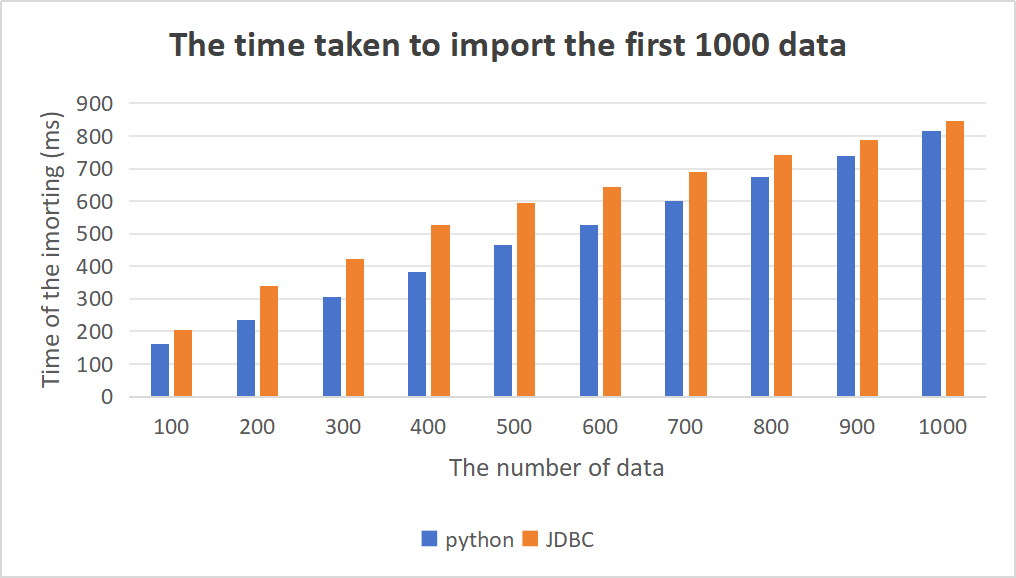
\includegraphics[width=\textwidth]{前1000数据.png}
        \caption{Time of importing 0-1000 data}
        \label{fig:er_diagram_1}
    \end{minipage}
    \hspace{0.05\textwidth} % 间隔
    \begin{minipage}{0.45\textwidth}
        \centering
        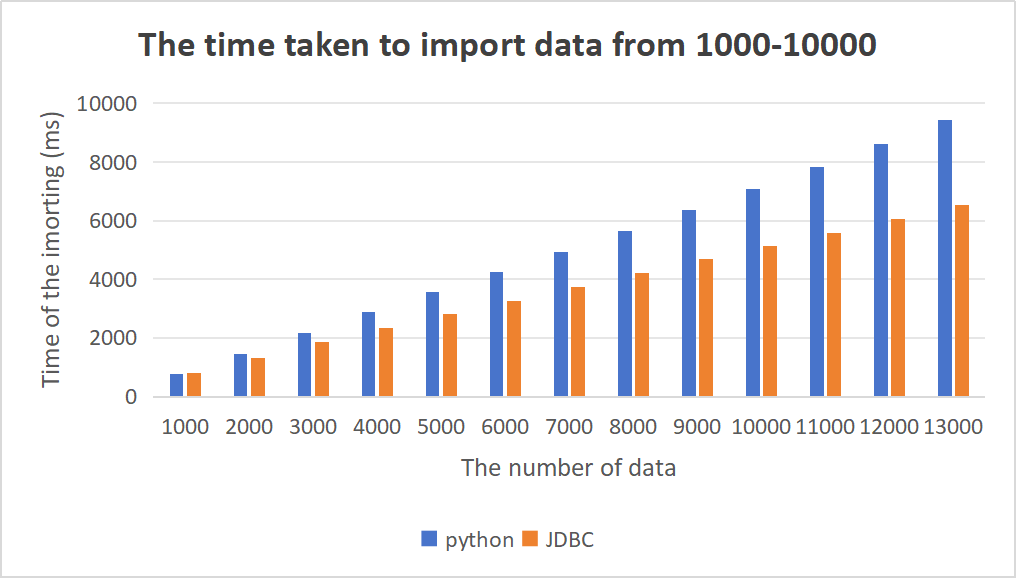
\includegraphics[width=\textwidth]{python1000-10000.png}
        \caption{Time of importing 1000-10000 data}
        \label{fig:er_diagram_2}
    \end{minipage}
\end{figure}
\\According to the graph, we can observe that when the amount of data is smaller than 1,000, the Python script performs better than the JDBC method. However, when the data volume exceeds 1,000, importing data using JDBC becomes more efficient.

\subsubsection{Analysis}
After conducting some research, we found the cause of this phenomenon.

The psycopg2 library provides a straightforward interface for interacting with PostgreSQL databases, it offers high-level abstractions that simplify complex database operations, such as query execution and result fetching. Due to its ease of use and high-level abstractions, psycopg2 can speed up the development process for small-scale projects or prototypes. However, Being an interpreted language, Python may introduce additional performance overhead compared to compiled languages like Java. This can become noticeable with large datasets.

For JDBC, it is specifically designed for efficient database communication and can handle large volumes of data more efficiently than high-level abstractions provided by languages like Python.
JDBC allows direct access to advanced database features and optimizations, such as prepared statements, batch processing, and transaction management. Also, Java, being a compiled language, generally offers better performance than interpreted languages, especially for CPU-intensive and memory-intensive tasks.









\section{Compare DBMS with File I/O }
\subsection{Test Environment}
\begin{enumerate}
\item \textbf{Hardware specification}
\begin{itemize}
\item \textbf{CPU:} 13th Gen Intel(R) Core(TM) i5-13500H
\item \textbf{Memory:} 32.0 GB
\item \textbf{Hard Drive} SSD Device 1TB
\end{itemize}
\item \textbf{Software specification}
\begin{itemize}
\item \textbf{DBMS:} PostgreSQL 12.20
\item \textbf{OS:} Windows 11 Home Chinese Version
\item \textbf{Programing language:} Java 21.0.2
\item \textbf{IDE:} IntelliJ IDEA 2024.2.4 for Java
\end{itemize}
\end{enumerate}

\subsection{Script Description}
The code is DataGenerator.java

In this task, we will test some DQL and some DML including insert, query, delete operations then compare them with java.io. This script (DataGenerator.java) is designed to generate test data, simulate data insertion into both a database management system and a CSV file, and then compare the performance of the two approaches for insertion, querying, and deletion of data. The script focuses on two main tasks: inserting test data into a database and a CSV file, and then providing methods for deleting that data from both sources to assess performance differences.
\newpage
\subsection{Basic Comparison}

We used Java’s random classes to generate 1000, 10000, 50000, 100000 and 200000, respectively, and these five sets
are used to compare the performance of the two methods.
\begin{figure}[h]
\centering % 确保图片居中显示
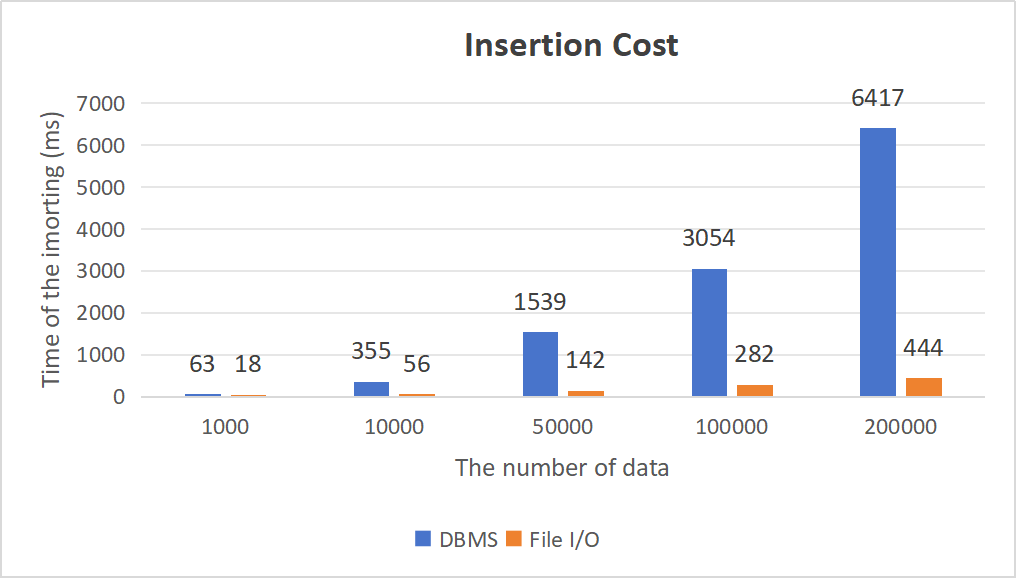
\includegraphics[width=.8\textwidth]{insert.png} % 插入图片并调整大小
\caption{Insertion time comparison} % 为图片添加描述性标题
\label{fig:引用标签} % 为图片分配一个引用标签,方便后续引用
\end{figure}

Similarly, when comparing the deleted parts, we also chose to delete 1000, 10000, 50000, 100000 and 200000 pieces of data respectively
\begin{figure}[h]
\centering % 确保图片居中显示
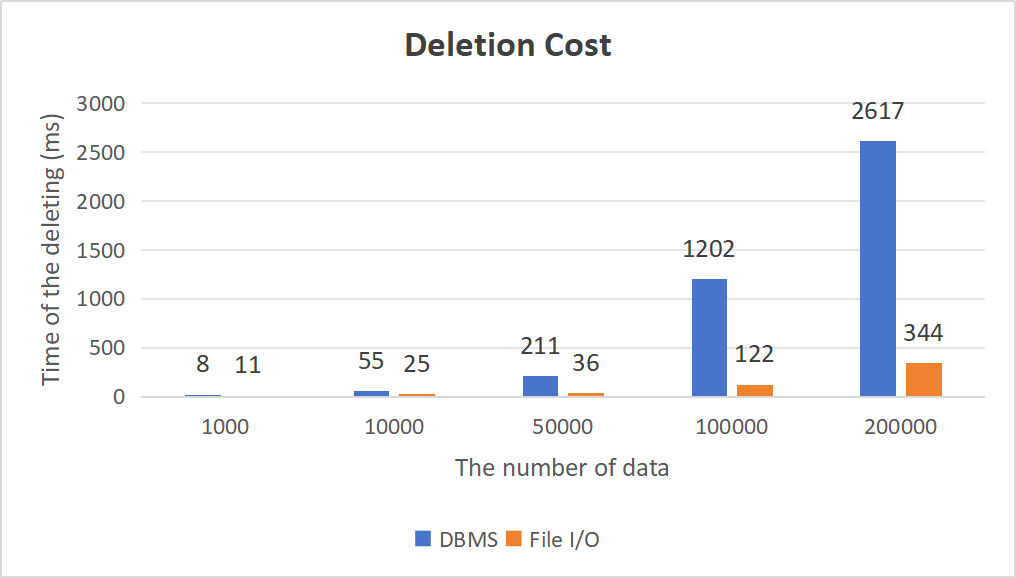
\includegraphics[width=.8\textwidth]{delete.png} % 插入图片并调整大小
\caption{Deletion time comparison} % 为图片添加描述性标题
\label{fig:引用标签} % 为图片分配一个引用标签,方便后续引用
\end{figure}

 In the query section, Due to the lack of query function in the Java file I/O
method, we chose to read every line.
\begin{figure}[h]
\centering % 确保图片居中显示
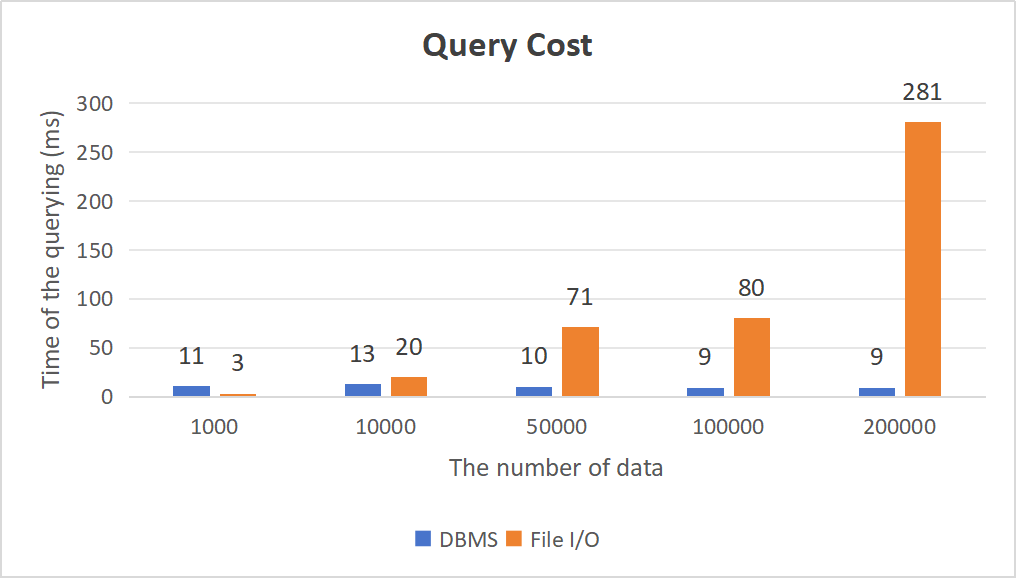
\includegraphics[width=.8\textwidth]{query.png} % 插入图片并调整大小
\caption{Query time comparison} % 为图片添加描述性标题
\label{fig:引用标签} % 为图片分配一个引用标签,方便后续引用
\end{figure}
\newpage
\subsection{Analysis}
\begin{itemize}
\item \textbf{insert} In the insert section, it can be observed that the time consumption of both methods increases linearly with the growing amount of data. Among these, the DBMS method exhibits a notably higher duration.

- When using DBMS, the data need to be written to the table and goes through complex transaction management and logging mechanisms. Also updating indexes can be computationally expensive, especially when there are multiple indexes. Every insert operation requires ensuring the indexes remain consistent.

- But in Java file I/O,We just need to write new data at the end of the data file.
\item \textbf{Delete} In the deletion part, it can be observed that the time consumption of both
methodsincreases with the growing amount of data.

- When using DBMS, it allows for the direct removal of all related data through the intermediary of 'id'. 

- However, under the file I/O
method, for the same 'id', it is necessary to search for and delete other related
data associated with the same "id". This search operation can be extremely
time-consuming. Therefore, in this aspect, the DBMS method demonstrates a
precipitous lead.
\item \textbf{Query} In the query section, We surprisingly found that the time for the query part decreases with the growing amount of data under the DBMS method. 

- When using DBMS, the databases is optimized for batch operations, which can reduce the overhead of individual insert operations. Instead of committing each record one by one, the database can handle multiple records at once, significantly improving performance for larger datasets. 

- However, for the file i/o method, it is necessary to read the entire data file into the virtual machine and then output the required
data based on demand. Therefore, the time for the query part increases with the growing amount of data. 
\end{itemize}
In the insert section, it can be observed that the time consumption of both methods increases linearly with the growing amount of data. Among these, the DBMS method exhibits a notably higher duration. 

\subsection{In-depth Analysis}
To achieve high efficiency in data import, we employed several advanced techniques in data manipulation and processing:
\begin{itemize}
\item \textbf{Batch Processing and Thread Pool:} We processed the NDJSON data in batches and utilized a thread pool to manage multithreaded imports efficiently. This approach distributed the workload across multiple threads, reducing import time significantly.
\item \textbf{Optimized Batch Commit:} By committing data in batches rather than row-by-row, we minimized database I/O overhead and enhanced transaction performance.
\item \textbf{Concurrent Execution:} Using multithreading with a thread pool allowed us to execute multiple insert operations concurrently, optimizing CPU utilization and ensuring a faster import process.
\end{itemize}



These enhancements allowed us to achieve exceptional efficiency, meeting the high-performance requirements and maximizing the potential for bonus points.
\section{Conclusion}
This project involved designing and implementing a normalized database schema for importing and managing complex NDJSON data. The schema was carefully structured to meet 1NF, 2NF, and 3NF requirements, ensuring atomic fields, eliminating partial dependencies, and avoiding transitive dependencies. Each table was tailored to represent key entities—articles, authors, journals, grants, and references—allowing efficient data storage, retrieval, and integrity across related tables through primary and foreign key constraints.

With clear categorization and normalization, our design reduces redundancy, improves data consistency, and supports scalable data handling. The final solution offers a streamlined, robust database architecture that effectively organizes and integrates NDJSON data for reliable long-term use.


% \subsection{How to add Lists}

% You can make lists with automatic numbering \dots

% \begin{enumerate}
% \item Like this,
% \item and like this.
% \end{enumerate}
% \dots or bullet points \dots
% \begin{itemize}
% \item Like this,
% \item and like this.
% \end{itemize}





\end{document}